\chapter{Waving Grass}

% GPU gems 1 chapter 7

A completely static terrain would appear quite lifeless. Some foliage
gently swaying in the wind would make the landscape seem more idyllic
and grass was therefore added.

Some considered rendering techniques for grass were

\begin{itemize}
\item Rendering grass straw textures on quads. This allows us to
  render several grass straws while only having to process 4
  vertices. Letting it wave in the wind is also easy as that only
  means moving the 2 top vertices. A problem however is that the
  illusion breaks down when viewed from above or on steep cliffs.
\item Modeling each grass straw. This technigue allows for very
  flexible grass with correct lighting. It is however very expensive
  to process all the vertices, so it's ususally used in conjunction
  with the above method for far away grass.
\item Rendering a volume texture containing the grass straws.
\end{itemize}

We opted for grass drawn onto quads, since it's easy to draw a quad of
grass on the screen and grass textures are easy to come by.

However the entire landscape can't simply be covered with millions of
quads of grass, as that would be extremely expensive to render, so
there are some design decisions to be made. Another problem with this
technique is that part of the grass texture is transparent, and
transparency isn't easy in the OpenGL 2.1 pipeline. A solution would
be depth peeling or z-sorting the straws, but for our purpose we
propose a much simpler method in the
\hyperref[sec:transparency]{Handling Transparency subsection}.

% @TODO reference GPU Gems 1

The basis of the grass implementation is Chapter 7 in GPU Gems 1. Here
they propose to draw the quads in objects with star patterns, to
achieve a grass effect independent of the cameras line of sight. Our
implementation does the same, but allows the user to specify how many
quads should be used used pr. star object. Setting this to 1
effectively disables the star pattern and simply renders random quads
of grass straws instead.

\section{Placing the grass}

As stated earlier we cannot simply draw the grass everywhere without
incurring a huge fps penalty, so instead we focus on drawing the grass
around the camera. We choose to draw it in a square around the camera,
but other shapes should be possible.

% explain algorithm

On \reffig{fig:grassTranslation} the basics of the algorithm can be
seen. We need to translate the square of grass centered around origo
to the camera. But we can't simply use the vector from origo to the
camera, since that would make the grass straws float along with the
camera. Instead we need grass straws exiting the square on one side to
overlap and appear on the other side. This can be achieved by ensuring
that grass objects are always moved by a multiplum of the grass
squares side's length, and is expressed in the following equation

\begin{displaymath}
    -halfSize \le position + size * n - eye \le halfSize, n \in N \\
\end{displaymath}

Focussing on the left hand side of the equation and remembering that
$n$ should be an integer, $n$ can be calculated as 

\begin{displaymath}
  \begin{array}{l}
    -halfSize \le position + size * n - eye \\
    \Updownarrow \\
    (eye - halfSize - position) / size \le n \\
    \Updownarrow \\
    n = \lceil (eye - halfSize - position) / size \rceil \\
    \Updownarrow \\
    n = \lceil (eye - position) / size - 0.5 \rceil \\
  \end{array}
\end{displaymath}

Now the new position of the grass straw is simply calculated by 

\begin{displaymath}
  newPos = position + size * n
\end{displaymath}

% And placing it in front of the camera


The grass quads have now succesfully ben placed in a square around the
camera, as can be seen on \reffig{fig:grassTranslation}. However most
of the straws still aren't inside the frustum. A small trick can be
applied to move more of the grass up in front of the camera. Instead
of placing the grass around the camera, it can be placed at a position
in front of it, relative to the cameras current direction. Since at
least half the grass square will be behind the camera, we choose to
move the camera position by the halfsize multiplied by the normalized
camera direction. This places the center of the grass in front of the
camera, but the border will never be in front of the camera. The
result is many more grass straws on the screen at the same vertex
processing cost.

% creation and one draw call

Since grass placed anywhere will now be translated to the camera, we
can create it anywhere we like. More importantly all the quads of
grass straws can now be drawn with one single draw call, and the
vertex shader will translate it to the camera. This removes a major
overhead we could have had if all quads should have been drawn
individually.

% Placing it on the heightmap and normal lookup

Our next hurdle is placing the grass straws on the terrain. Since
we're continuesly translating the grass quads, we can't know their
correct height at creation time and must therefore calculate it in the
vertex shader. We therefore calculate a texture coordinate from the
grass position and use that to lookup into the heightmap texture,
where we can find the correct height for the grass. To ensure that the
terrain and grass are equally lighted (lit?), we use the same
procedure to lookup into the heightmaps normalmap.

% not on sand or snow.

The last part of the grass placement is to keep it off the sand, snow
and steep cliffs. To this end we pass along the center of the grass
straw to the vertex shader. The center is then subjected to the same
translations as the vertex position. Wether or not the grass straws
should be visible can then be estimated from the height of the
center. If the center is too low the grass is on sand and should not
be visible, likewise if the center is too high it is snow. A similar
scheme is used for deciding if the grass is above cliff, where the
height is replaced by the normal.

The reason for using the center of the grass objects is that while one
side of the quad may be placed perfectly legal, the other side could
be placed on sand or snow. In order to collapse the grass objects we
needed a constant variable across the objects and that was the center.


\section{Waving in the wind}

Our animation algorithm is the same as the one proposed in section
7.4.4 of GPU Gems 1, where the grass objects center is used to create
'local chaos'. This means that all the grass can still be drawn with
only one draw call, texture are minimally distorted since the vertices
always have the same distance to their neighbours and the local chaos
creates a more natural wave effect. Of the two cons to the approach
only one of them applies to our implementation. The first con, which
is that extra uniform data is required to hold the center of the grass
object, doesn't apply ion this case, since the center was needed
anyway. The second con does apply to our shader, namely that the
complexity of the animation algorithm is limited in order to minimize
the cost of the shader. The wave therefore is just a simple cosine
function applied to the two top vertices, distinguished by their
texture coordinate.


\section{Handling Transparency}\label{sec:transparency}

% Discarding seethrough texture (how to avoid z sorting and rendering
% everything with one draw call)

With the grass placed on the terrain, texture transparency needs to be
handled. The grass straw texture can be seen in
\reffig{fig:grassStraws}. Since everything is drawn with one draw
call, z-sorting every frame isn't an option. Instead the transparency
and drawing order issue is completely ignored, by only rendering
completely opaque fragments or discarding them. This is done in the
fragment shader, where colors with alpha values below a certain value
are simply discarded. The reason for not just discarding everything
stictly below 1 is that mipmapping has to be taken into account. If 2
opague and 2 transparent pixels are combined in a lower mipmap layer,
that would yield an alpha of 0.5, but the fragment should perhaps
still be rendered. In practice we found that discarding alphas below
0.6 works well with the grass straw texture.

\begin{figure}
  \label{fig:grassStraws}
  \centering
  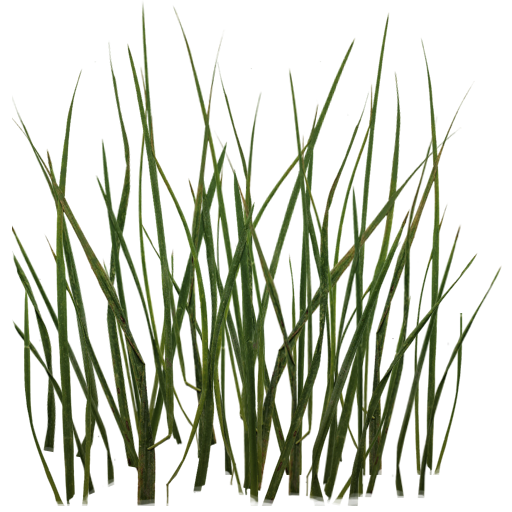
\includegraphics[width=5cm]{grassStraw}
  \caption{The grass straws.}
\end{figure}

% Simple diffuse lighting, no specular.






%%% Local Variables:
%%% mode: latex
%%% TeX-master: t
%%% TeX-PDF-mode: t
%%% End:
